% !TeX root = ../libro.tex
% !TeX encoding = utf8
\chapter{Diseño, implementación y despliegue del simulador}
\section{Introducción}
En este apartado vamos a detallar la implementación de un simulador mediante tecnología web para mostrar la aplicación y utilidad de este trabajo de una forma mucho más gráfica y dinámica, con la posibilidad de cambiar los parámetros del edificio a nuestro gusto y ver cómo afectan a las distintas temperaturas del edificio.

Veremos el proceso y desarrollo del simulador, realizando un análisis del diseño del proyecto, incluyendo los distintos tipos de requisitos junto con el proceso de verificación, para el desarrollo hemos utilizado tecnologías actuales que podremos encontrar en cualquier proyecto de desarrollo de las principales empresas hoy en día, además veremos los aspectos más importantes en el proceso de creación del backend y frontend, detallando todos los pasos que hemos seguido tanto en el diseño como en la implementación, mostraremos algunos ejemplos de casos de uso del simulador para comprobar su correcto funcionamiento comparándolo con la parte teórica, además, al final se discutirán posibles mejoras y actualizaciones que se podrían realizar sobre el proyecto a futuro.

El objetivo es que sea accesible para cualquier usuario, y para ello la interfaz será muy intuitiva y fácil de entender, además incluiremos en el \autoref{ap:apendice1} una pequeña guía de instalación y acceso del simulador, de tal forma que cualquiera pueda utilizarlo y probarlo.
\section{Tecnologías utilizadas}
A continuación vamos a enumerar y explicar los principales motivos y características acerca de las tecnologías que hemos utilizado, incluyendo el enlace a sus páginas web oficiales. Empezamos por las que hemos requerido para desarrollar el backend:
\begin{itemize}
	\item \href{https://www.python.org}{Python}. Además de porque tiene una comunidad muy amplia, la cual nos permite encontrar feedback rápidamente sobre cualquier duda o problema que tengamos, es uno de los lenguajes más utilizados para ciencia de datos, IA y cálculo, por lo que existen muchas librerías para simplificar la implementación de nuestros sistemas de ecuaciones diferenciales. Aunque otra opción es utilizar Java o en $C$++, sería más complejo realizar el cálculo de las ecuaciones diferenciales además del manejo de los datos, así que por las necesidades del proyecto hemos decidido utilizar Python. Las principales bibliotecas que hemos utilizado para el cálculo matemático son \href{https://numpy.org}{Numpy} y \href{https://scipy.org}{Scipy}.
	\item \href{https://flask.palletsprojects.com/en/3.0.x/}{Flask}. Es un framework para Python muy popular utilizado comúnmente para crear aplicaciones web, y sobre todo, servicios web. Nos hemos decantado por su uso debido al hecho de ser gratuito y de código abierto, además de su sencillo uso.
	\item \href{https://www.json.org/json-es.html}{JSON}. Notación estándar para el intercambio de información entre los servicios y las aplicaciones. Está basado en un subconjunto del lenguaje JavaScript, y una característica muy importante es que no depende del lenguaje que se utilice, por lo que es ideal para el intercambio de datos.
	\item \href{https://www.openapis.org}{OpenAPI}. Es una notación estándar para describir y compartir con otros usuarios (desarrolladores, comunidad) nuestro servicio web (resolución de sistemas de ecuaciones diferenciales).
\end{itemize}
En cuanto al desarrollo del frontend hemos utilizado:
\begin{itemize}
	\item \href{https://es.react.dev}{React}. Es una de las librerías más populares de JavaScript, está diseñada para crear interfaces de usuario con el objetivo de facilitar el desarrollo de aplicaciones en una sola página. Tiene un alto rendimiento y permite infundir código HTML con JavaScript. Aplicaciones muy populares como Facebook, Netflix, DropBox, Instagram o Paypal usan React, y es por ello que es tan importante y nos hemos querido familiarizar con ella en este trabajo. Además, es mantenida por Facebook y la comunidad de software libre.
	\item \href{https://www.highcharts.com}{Highcharts}. Es una librería escrita en JavaScript para generar gráficos interactivos en aplicaciones web, soporta una gran variedad de gráficos y en nuestro caso la utilizaremos para mostrar el resultado final.
	\item \href{https://getbootstrap.com}{Bootstrap}. Es un framework que permite a los desarrolladores web darle forma a un sitio web y adaptarlo a las necesidades de los usuarios, nosotros lo hemos utilizado para mejorar el diseño de la página.
	\item \href{https://ant.design}{Ant Design}. Es una biblioteca React UI (User Interface), que como su nombre indica, permite construir interfaces de usuario con un elegante diseño, la hemos compaginado con Bootstrap para mejorar el diseño de la página.
\end{itemize}
En el diagrama de la \autoref{fig:arquitectura} podemos ver la arquitectura que sigue el simulador junto con los logos de las principales tecnologías que hemos utilizado tanto para el frontend como para el backend.
\begin{figure}[h!]
	\centering
	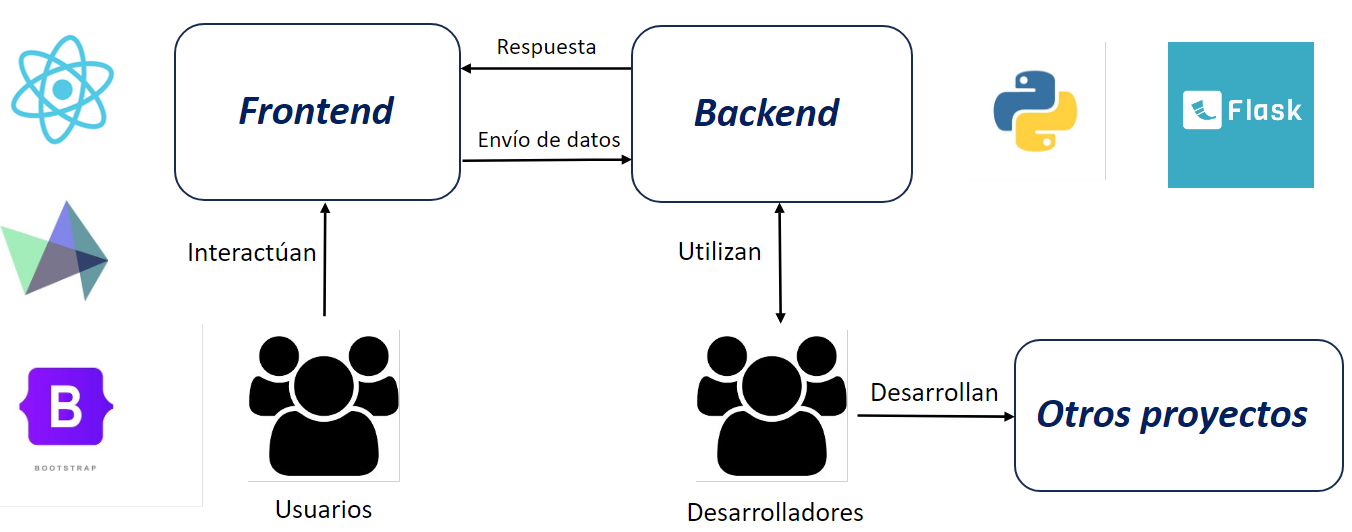
\includegraphics[width=\textwidth]{diagrama}
	\caption{Arquitectura del simulador}
	\label{fig:arquitectura}
\end{figure}
\section{Diseño}
\subsection{Análisis de requisitos}
\subsubsection{Requisitos funcionales}
Los requerimientos funcionales son aquellos que vienen establecidos por las funcionalidades del sistema, es decir, definen el comportamiento interno del software.
\begin{itemize}
	\item \textbf{RF$1$}. El sistema deberá ser capaz de crear un nuevo edificio. El  usuario deberá rellenar un formulario que debe ser comprobado por el software.
	\item \textbf{RF$2$}. El sistema deberá ser capaz de leer los datos del formulario y crear y resolver un sistema de ecuaciones diferenciales correspondiente, proporcionando la solución en el formato adecuado.
	\item \textbf{RF$3$}. El sistema deberá ser capaz de borrar un edificio que se esté generando para volver al estado inicial. El  usuario podrá seleccionar un botón de Reset para ello.
	\item \textbf{RF$4$}. El sistema deberá poder generar un informe con los datos de las temperaturas de las habitaciones durante el día. Dicho informe se generará en formato JSON.
	\item \textbf{RF$5$}. El sistema deberá poder generar una gráfica con las temperaturas de las habitaciones durante el día además de la temperatura exterior.
\end{itemize}
\subsubsection{Requisitos no funcionales}
Los requisitos no funcionales son aquellos que imponen restricciones sobre el diseño o la implementación.\\

\noindent \textbf{Usabilidad.}
\begin{itemize}
	\item \textbf{RN$1$}. La navegación por la web debe ser intuitiva y estar dotada de instrucciones para los usuarios y así facilitar la interacción de los usuarios con la interfaz.
	\item \textbf{RN$2$}. Se deberán comunicar avisos cuando, por ejemplo, se cometa un error al introducir datos en el formulario, indicando la forma correcta de introducir los datos.
\end{itemize}
\textbf{Rendimiento.}
\begin{itemize}
	\item \textbf{RN$3$}. Se debe tener en cuenta el número de habitaciones que tenga el edificio, para no generar un sistema de ecuaciones excesivamente complejo y que dificulte la computación.
	\item \textbf{RN$4$}. El sistema ha de ser capaz de realizar todas las conexiones sin que esto repercuta en el tiempo de espera ni en el rendimiento.
\end{itemize}
\textbf{Soporte.}
\begin{itemize}
	\item \textbf{RN$5$}. Cuando un usuario genere un edificio, debe facilitarnos toda la información necesaria para calcular las temperaturas internas. Deberemos adaptarla para que sea compatible con el formato del sistema de ecuaciones diferenciales correspondiente.
\end{itemize}
\textbf{Organizativos.}
\begin{itemize}
	\item \textbf{RN$6$}. La API se desarrollará utilizando como lenguaje de programación Python y el framework Flask. Por otro lado, para el desarrollo del frontend se utilizará React, que permitirá aportar dinamicidad al sistema.
\end{itemize}
\subsection{Verificación}
Vamos a verificar que el sistema funciona correctamente, es decir, que cumple con los requisitos funcionales y no funcionales descritos anteriormente:
\begin{figure}[h!]
	\centering
	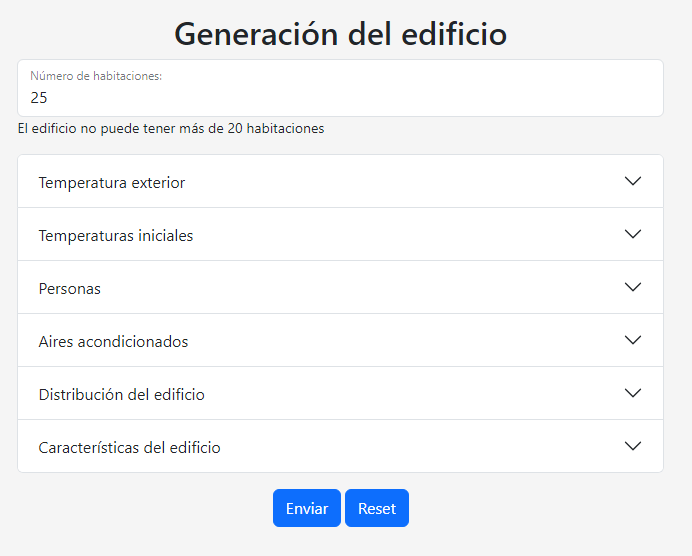
\includegraphics[width=0.8\textwidth]{form20habs}
	\caption{Formulario intentando introducir 25 habitaciones}
	\label{fig:20habs}
\end{figure}

\begin{itemize}
	\item En la \autoref{fig:20habs} podemos ver el formulario que debe rellenar el usuario para crear un nuevo edificio, cumpliendo así el primer requisito \textbf{RF}$1$, además aparece el botón para poder hacer Reset, de forma que podamos borrar el edificio actual y generar uno nuevo, como se indica en \textbf{RF}$3$, por otro lado vemos cómo tenemos avisos en el formulario que se generan de forma dinámica para ayudar al usuario a introducir los datos de forma correcta, lo que verifica los requisitos \textbf{RN}$1$ y \textbf{RN}$2$, en cuanto al apartado de rendimiento, hemos puesto un número máximo de 20 habitaciones en el edificio para no colapsar el sistema, y todos los cálculos y conexiones se hacen muy rápidamente, en cuestión de milisegundos, verificando \textbf{RN}$3$ y \textbf{RN}$4$, por último, también se verifica \textbf{RN}$5$, ya que como se ve en \autoref{fig:sistema}, el sistema es capaz de generar el sistema a partir de los datos introducidos por el usuario.
	\item Una vez se han leído los datos del formulario, se crea el sistema de ecuaciones diferenciales asociado como podemos ver en la \autoref{fig:sistema}, cumpliendo \textbf{RF}$2$.
	\item En la \autoref{fig:parte_derecha}, se puede ver que podemos descargar la solución en formato JSON, además de la gráfica con las temperaturas internas de las distintas habitaciones además de la externa, verificando los requisitos \textbf{RF}$4$ y \textbf{RF}$5$.
	\item Efectivamente, se ha utilizado Python y Flask para el desarrollo del backend, y React para el frontend, verificando así el requisito \textbf{RN$6$}. En la \autoref{fig:arquitectura} se pueden ver las principales tecnologías que se han utilizado.
\end{itemize}

\begin{figure}[h!]
	\centering
	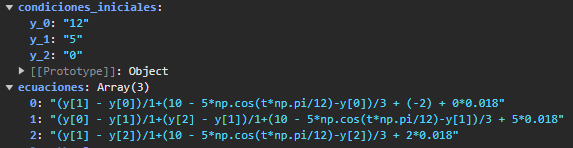
\includegraphics[width=\textwidth]{sistema}
	\caption{Sistema de ecuaciones diferenciales creado a partir del edificio}
	\label{fig:sistema}
\end{figure}

\section{Frontend}
\subsection{Idea inicial del diseño}
\begin{figure}[h!]
	\centering
	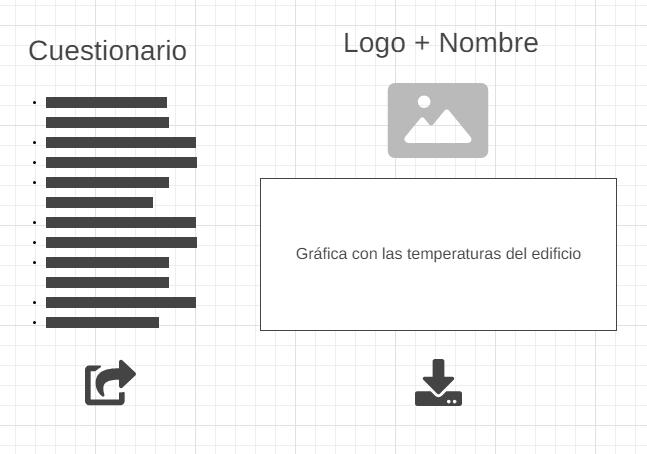
\includegraphics[width=0.8\textwidth]{mockup}
	\caption{Idea principal del diseño del simulador}
	\label{fig:mockup}
\end{figure}
En la \autoref{fig:mockup} podemos ver un wireframe del diseño propuesto para el frontend antes de realizar la implementación. Para recoger los datos y parámetros del edificio hemos decidido utilizar un cuestionario sencillo, y justo debajo tendrá un botón para enviar los datos a la API.

En el lado derecho tendremos un logo o nombre del simulador con el objetivo de darle una seña de identidad al proyecto, y justo debajo una gráfica con la solución al problema, es decir, las temperaturas de las habitaciones internas del edificio, que se mostrarán como respuesta de la API cuando le demos al botón de enviar. Por último, un botón para descargar los resultados en formato JSON, por si algún desarrollador quiere utilizarlo en otro proyecto.
\subsection{Desarrollo y diseño}
El objetivo principal del frontend es tener una herramienta web, visual y atractiva, que mediante una serie de parámetros, nos permita obtener los valores correspondientes a la resolución de nuestros sistemas de ecuaciones diferenciales, para que cualquier tipo de usuario pueda hacer uso de esta herramienta sin tener un conocimiento experto relacionado con las matemáticas ni la informática.

\begin{figure}[h!]
	\centering
	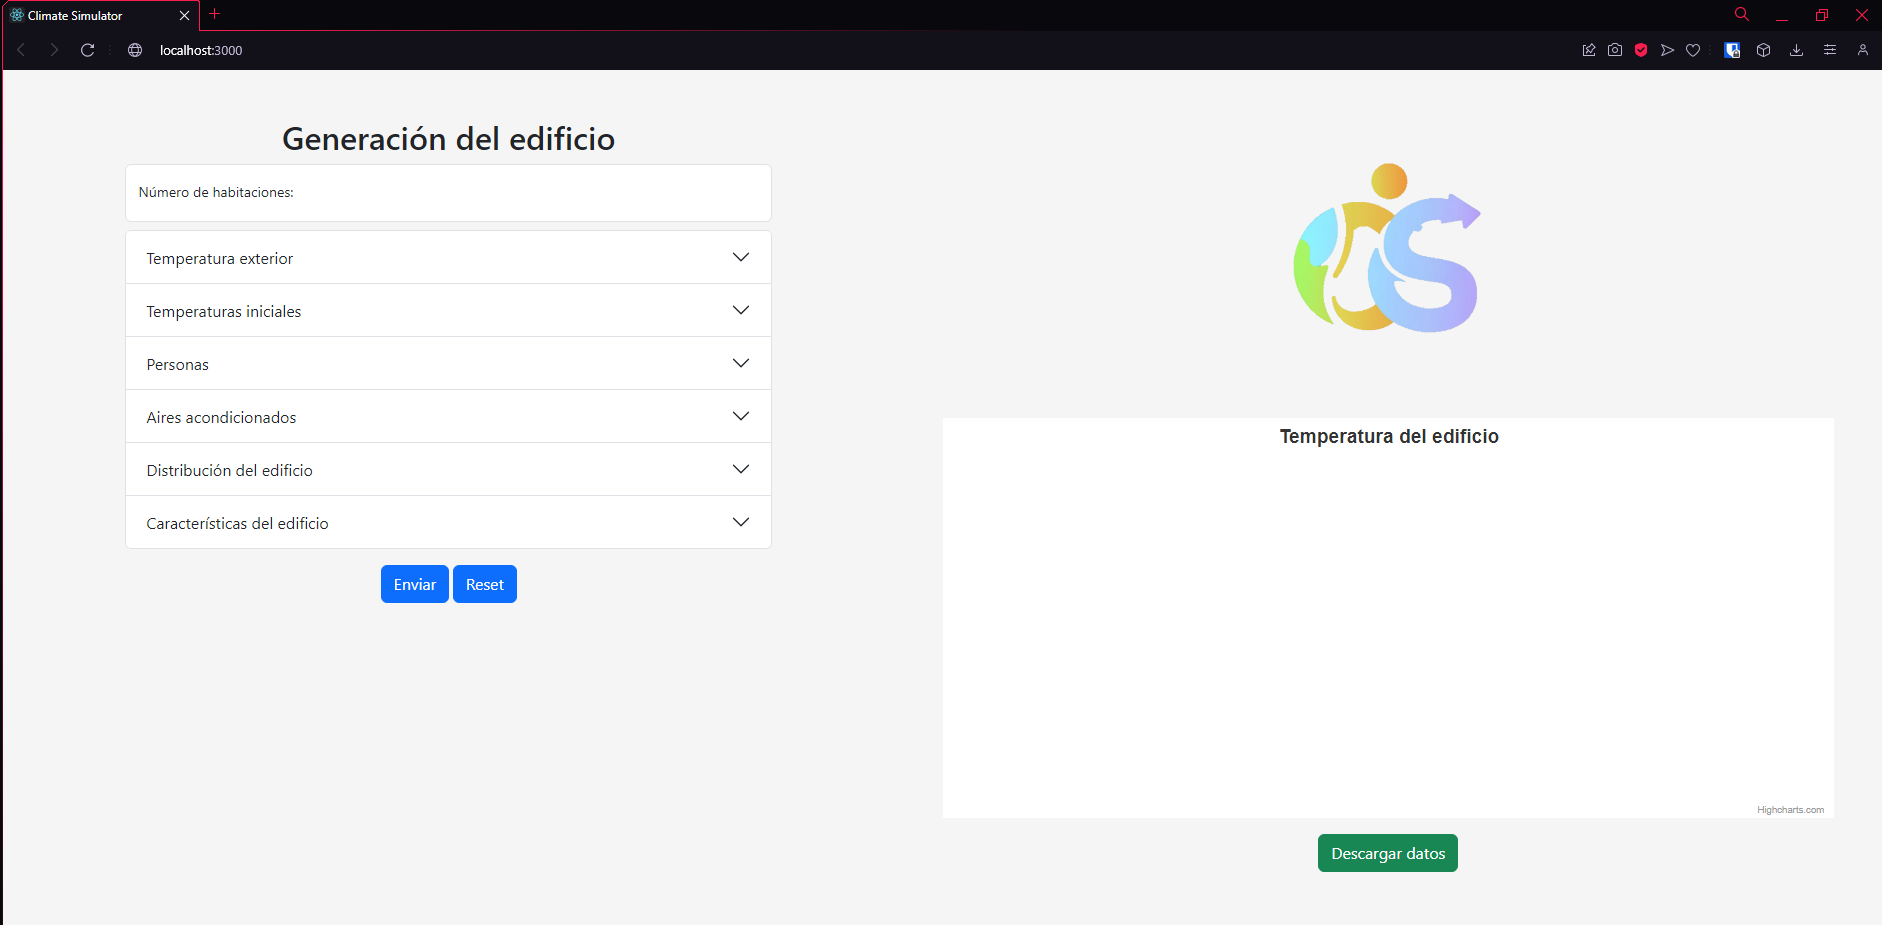
\includegraphics[width=\textwidth]{pag_web}
	\caption{Frontend del simulador}
	\label{fig:pag_web}
\end{figure}

Nada más abrir la página nos encontramos con el aspecto que podemos ver en la \autoref{fig:pag_web}, donde a la izquierda tenemos un formulario dinámico que nos permite generar el edificio con todos los parámetros necesarios, y es que los campos del formulario varían en tiempo real según el número de habitaciones, esto es posible gracias a que estamos utilizando React. Para mejorar el diseño y estilo del formulario hemos utilizado tanto Ant Design como Bootstrap, con el objetivo de hacer una interfaz más agradable para el usuario.
\begin{figure}[h!]
	\centering
	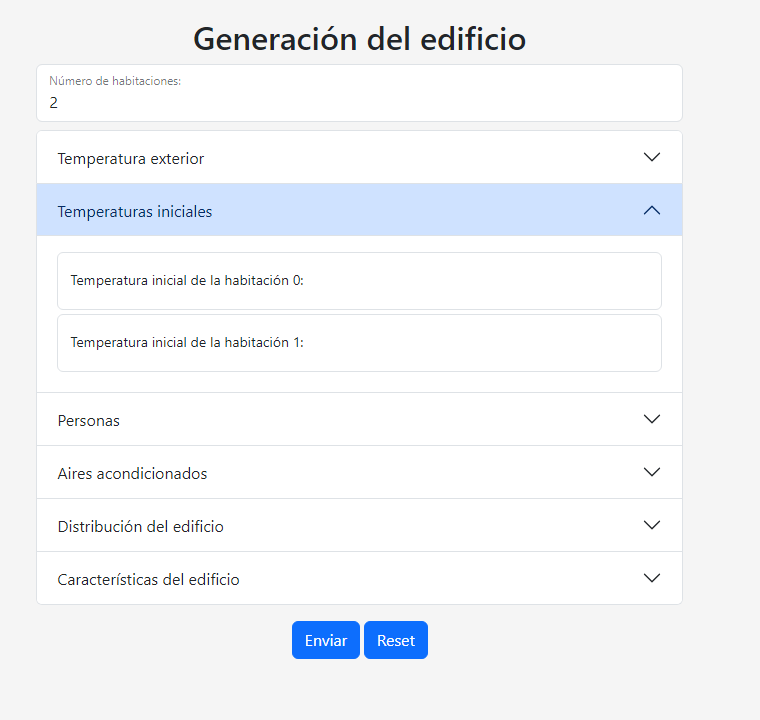
\includegraphics[width=0.7\textwidth]{formulario_2habs}
	\caption{Formulario introducir $2$ habitaciones}
	\label{fig:form_2habs}
\end{figure}
En la \autoref{fig:form_2habs} podemos ver cómo se incluyen $2$ habitaciones en el desplegable al haber introducido que el edificio tendrá $2$ habitaciones, y si cambiamos el número de habitaciones, el formulario cambia dinámicamente.

Para añadir la temperatura exterior, hemos incluido dos opciones, que podremos cambiar haciendo click en la barra superior del campo:
\begin{figure}[h!]
	\centering
	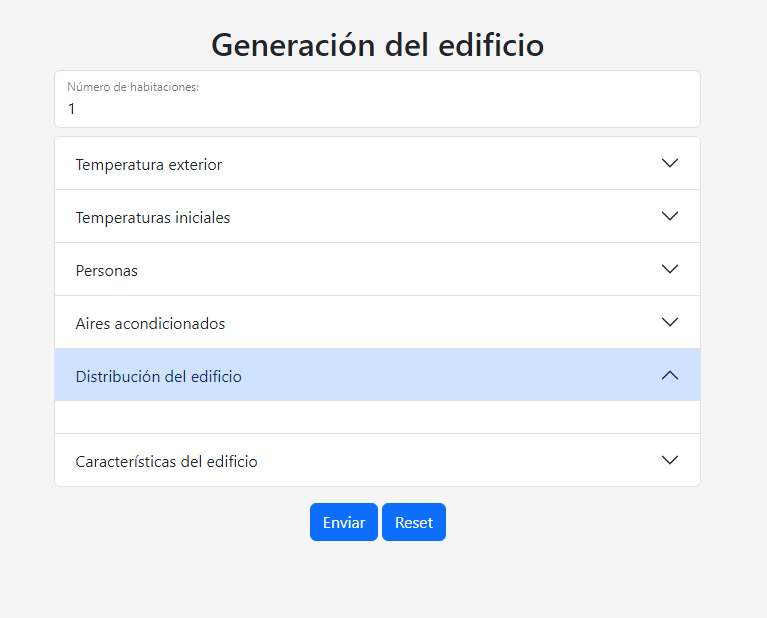
\includegraphics[width=0.75\textwidth]{una_hab}
	\caption{Formulario con $1$ habitación}
	\label{fig:una_hab}
\end{figure}
\begin{itemize}
	\item Opción $1$: Aquí podremos incluir directamente la función que tendrá la temperatura exterior durante las $24$ horas, está pensada para usuarios expertos en el tema. La función debe ser leída por la biblioteca $NumPy$ de Python, luego tendremos que usar expresiones como por ejemplo: $5 - 10*np.cos(t*np.pi/12)$
	\item Opción $2$: Podremos indicar la temperatura media del día y además cuánta variación tendrá, por ejemplo, si ponemos temperatura media de $10 \celsius$, y variación de $5$, entonces la temperatura variará entre $5 \celsius -15 \celsius$ grados, esta opción está pensada para que cualquier tipo de usuario pueda introducir la temperatura externa, sin necesidad de tener un conocimiento experto.
\end{itemize}

Otro detalle a tener en cuenta es que si ponemos sólo una habitación, no nos aparecerá la distribución del edificio, ya que no tendría sentido, como podemos ver en la \autoref{fig:una_hab}.

Al final tenemos dos botones tanto para enviar el formulario y obtener inmediatamente la gráfica con las temperaturas a la derecha, o para resetear el formulario por si queremos empezar de nuevo a crear el edificio.
\begin{figure}[h!]
	\centering
	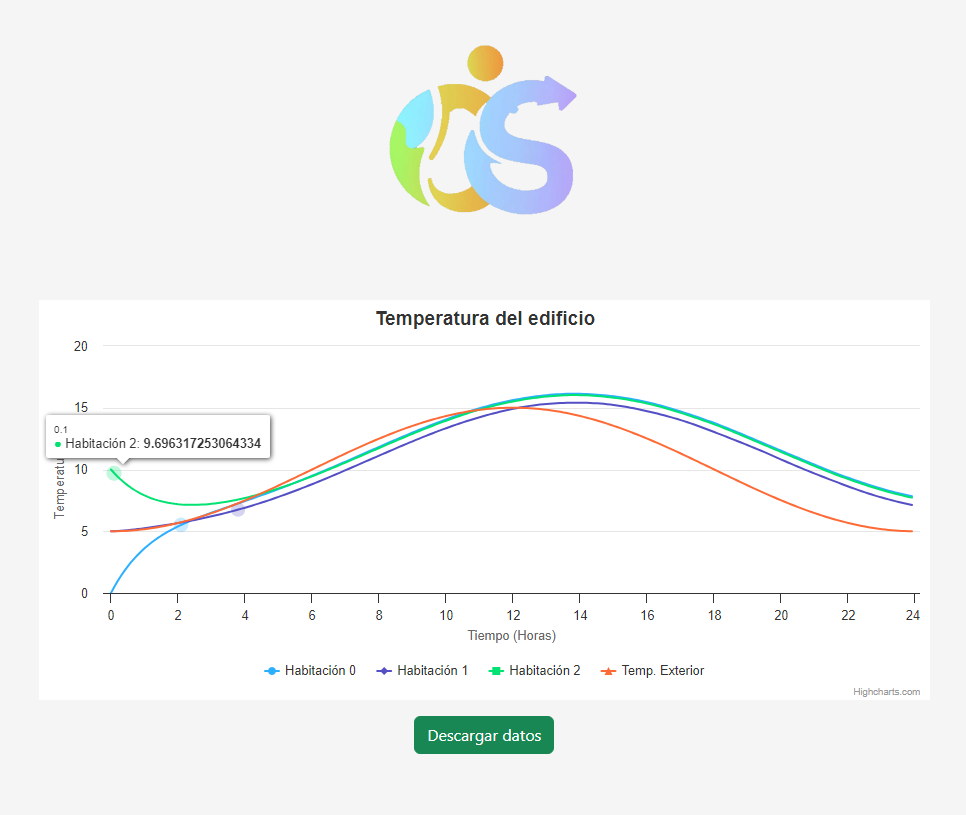
\includegraphics[width=\textwidth]{parte_derecha}
	\caption{Parte derecha de la página}
	\label{fig:parte_derecha}
\end{figure}

Ahora pasando a la parte derecha, tenemos en primer lugar el logo que hemos decidido añadir a la página, esto le aporta una identidad al proyecto aparte de ser más atractivo, justo debajo tenemos la solución al problema, es decir, una gráfica que hemos incluido gracias a Highcharts donde podemos ver las temperaturas de cada habitación, además de la temperatura externa para cada hora del día, y si pasamos el cursor por encima podemos ver el valor numérico de la temperatura en una hora determinada, todo esto se muestra en la \autoref{fig:parte_derecha}.

Por último, hemos incluido justo debajo un botón verde que nos permite descargar los datos de las temperaturas obtenidas en formato JSON, esta es una funcionalidad muy interesante que nos permite utilizar los resultados como posible entrada para otro programa por si fuesen necesarios.

\section{Desarrollo del Backend}
Por las ventajas ya mencionadas, para la implementación del backend de nuestra propuesta se va seguir la filosofía RESTful, ya que es la más utilizada hoy en día, esto quiere decir que nuestro servicio web implementa una arquitectura de REST, la cual sirve para estandarizar comunicaciones web entre sistemas, logrando que se entiendan mucho mejor entre ellos. Se basa en que el cliente envía peticiones para recuperar o modificar recursos, y el servidor responde con el resultado, que puede ser con los datos que hemos pedido o el estado de la petición.

\begin{figure}[h!]
	\centering
	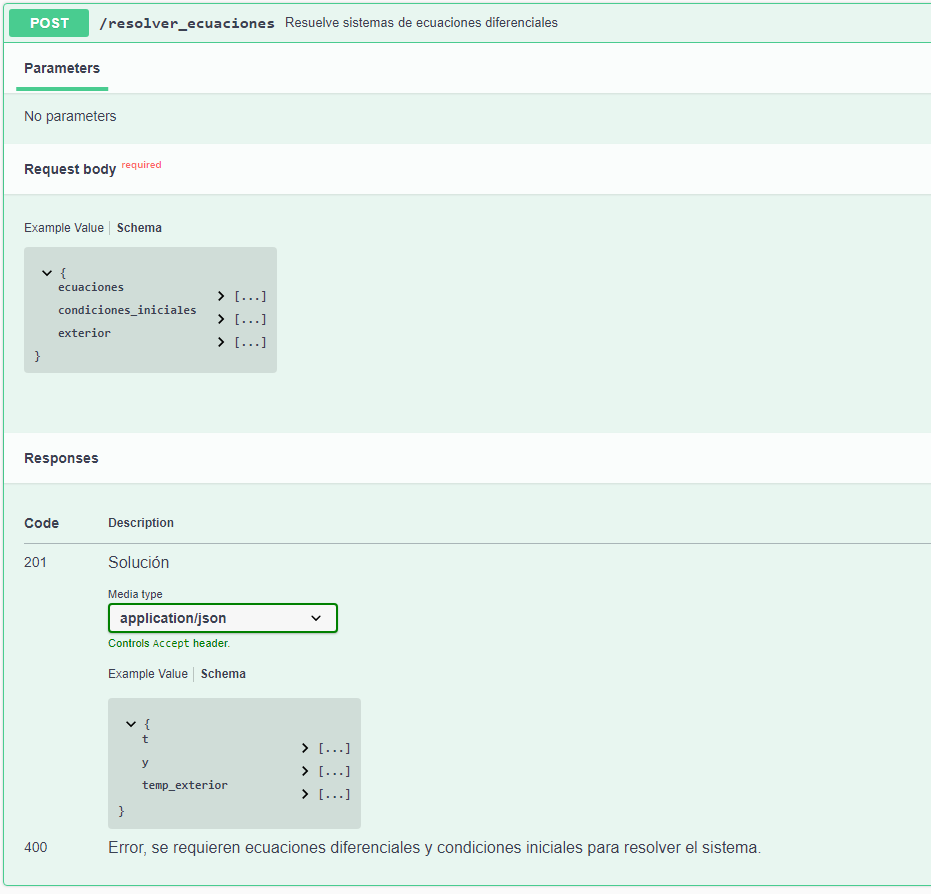
\includegraphics[width=\textwidth]{openapi}
	\caption{Especificación OpenAPI}
	\label{fig:openapi}
\end{figure}

Todo el desarrollo lo hemos realizado utilizando el lenguaje de programación Python, y nos hemos servido de Flask para crear el servicio web.

El objetivo principal de nuestra API es resolver sistemas de ecuaciones diferenciales, para ello recibimos del servidor web las ecuaciones, las condiciones iniciales y la función que representa la temperatura exterior del edificio, y devuelve un vector formado por:
\begin{itemize}
	\item Un vector con los puntos que representarán el tiempo en el eje $X$ (de $0$ a $24$ horas).
	\item Un vector en el que cada componente contiene otro vector con las temperaturas de cada habitación en cada instante de tiempo (los puntos del primer vector).
	\item Un último vector formado por la temperatura externa en cada instante de tiempo.
\end{itemize} 
La información es devuelta por el backend como respuesta al frontend, donde se construirá la gráfica final con los resultados obtenidos.

Además, vamos a añadir el estándar de OpenAPI, que nos permite visualizar los métodos de la API para que cualquier programador o persona interesada pueda ver de forma esquemática el uso y funcionamiento detallado de cada uno de los métodos. Un detalle muy importante es que es independiente del lenguaje de programación con el que esté desarrollada la API. En la \autoref{fig:openapi} podemos ver cómo queda la documentación, la cual es accesible para todo el mundo. Podemos ver el archivo con la especificación OpenAPI completa en \autoref{ap:especificacion}.

\section{Casos de uso}
\subsection{Ejemplo con 3 habitaciones que vimos en la \autoref{fig:edif3}}
Siguiendo el modelo de edificio que tomamos en el ejemplo de la \autoref{fig:edif3}, vamos a rellenar el formulario con los siguientes datos:
\begin{itemize}
	\item Número de habitaciones: $3$
	\item Temperatura exterior: $5 - 10\cdot cos(t\cdot \pi/12)$
	\item Temperatura inicial de las habitaciones: $20,10,15$
	\item Cantidad de personas en las habitaciones: $1,10,0$
	\item Aires acondicionados en las habitaciones $0$ y $2$
	\item Distribución del edificio: 
	\begin{itemize}
		\item Habitaciones contiguas a la habitación $0$: $1,2$
		\item Habitaciones contiguas a la habitación $1$: $0$
		\item Habitaciones contiguas a la habitación $2$: $0$
	\end{itemize}
	\item Características del edificio:
	\begin{itemize}
		\item Constante de transferencia entre habitaciones: $5$
		\item Constante de transferencia con el exterior: $3$
		\item Calor generado por el aire acondicionado: $-8\celsius / 5h$
	\end{itemize}
\end{itemize}
Al introducir los datos en el formulario y hacer click en el botón Enviar, obtenemos la solución al problema, la cual coincide con la que vimos en \autoref{fig:graf_sol3}:
\begin{figure}[h!]
	\centering
	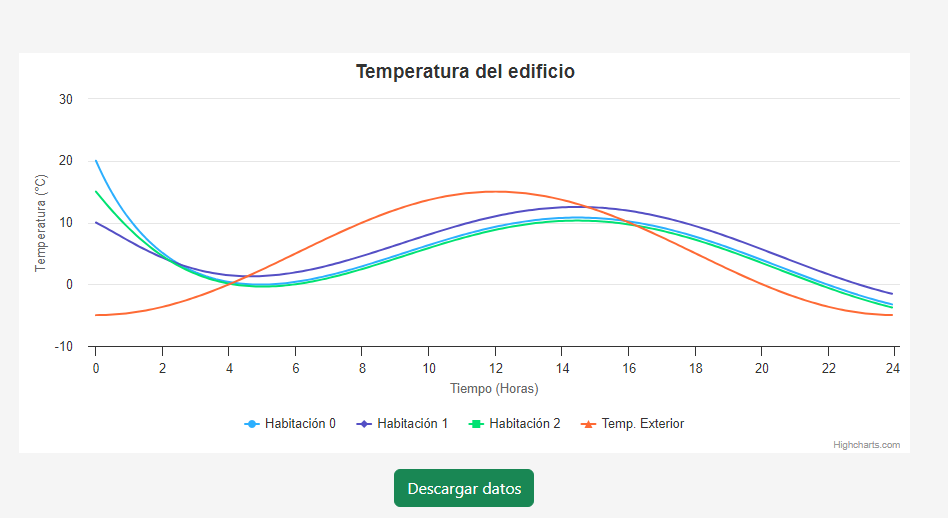
\includegraphics[width=\textwidth]{uso1}
	\caption{Temperaturas internas del edificio}
	\label{fig:caso1}
\end{figure}
\subsection{Ejemplo con 6 habitaciones}
Vamos a diseñar un nuevo edificio algo más elaborado, que constará de 6 habitaciones y seguirá la estructura que podemos ver en la \autoref{fig:edificio6}.
\begin{figure}[h!]
	\centering
	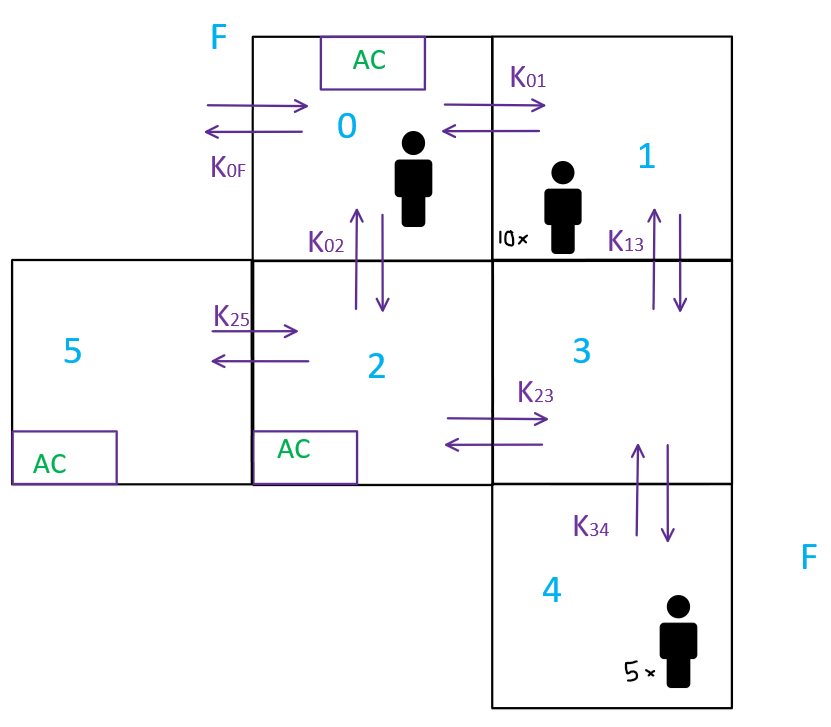
\includegraphics[width=0.8\textwidth]{edificio_6habs}
	\caption{Estructura del edificio con 6 habitaciones}
	\label{fig:edificio6}
\end{figure}
Vamos a introducir los siguientes datos en el formulario que corresponden con nuestro edificio:
\begin{itemize}
	\item Número de habitaciones: $6$
	\item Temperatura exterior: $20 - 15\cdot cos(t\cdot \pi/12)$
	\item Temperatura inicial de las habitaciones: $20,10,15,5,5,12$
	\item Cantidad de personas en las habitaciones: $1,10,0,0,5,0$
	\item Aires acondicionados en las habitaciones $0$, $2$ y $5$
	\item Distribución del edificio: 
	\begin{itemize}
		\item Habitaciones contiguas a la habitación $0$: $1,2$
		\item Habitaciones contiguas a la habitación $1$: $0,3$
		\item Habitaciones contiguas a la habitación $2$: $0,3,5$
		\item Habitaciones contiguas a la habitación $3$: $1,2,4$
		\item Habitaciones contiguas a la habitación $4$: $3$
		\item Habitaciones contiguas a la habitación $5$: $2$
	\end{itemize}
	\item Características del edificio:
	\begin{itemize}
		\item Constante de transferencia entre habitaciones: $3$
		\item Constante de transferencia con el exterior: $8$
		\item Calor generado por el aire acondicionado: $-4\celsius / h$
	\end{itemize}
\end{itemize}
Al introducir los datos en el formulario y hacer click en el botón Enviar, obtenemos la solución al problema, como podemos ver en la \autoref{fig:caso2}. Podemos observar que el edificio tiene un gran aislamiento con el exterior, y es por ello que las temperaturas de las habitaciones no se ven prácticamente influenciadas por la temperatura exterior, además de las altas temperaturas exteriores y tener un aire acondicionado que genera bastante frío, podríamos estar ante un escenario típico de verano.
\begin{figure}[h!]
	\centering
	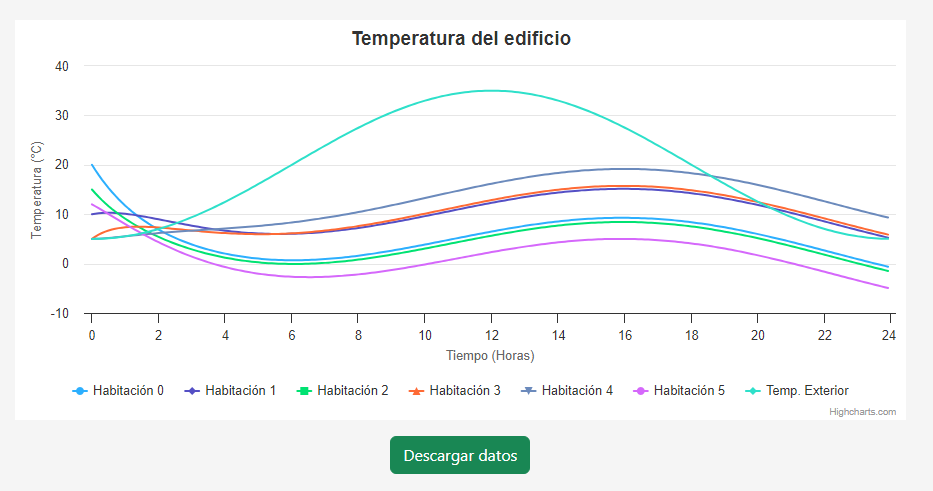
\includegraphics[width=\textwidth]{sol_6habs}
	\caption{Temperaturas internas del edificio con 6 habitaciones}
	\label{fig:caso2}
\end{figure}




\endinput
%------------------------------------------------------------------------------------
% FIN DEL CAPÍTULO. 
%----------------------------------------------------------------------------------
-